\documentclass[tikz]{standalone}
\usetikzlibrary{calc,trees,positioning,arrows,chains,shapes.geometric,%
    decorations.pathreplacing,decorations.pathmorphing,shapes,%
    matrix,shapes.symbols,fit}

\pgfdeclarelayer{back}
\pgfsetlayers{back,main}

\makeatletter
\tikzset{
  fitting node/.style={
    inner sep=0pt,
    fill=none,
    draw=none,
    reset transform,
    fit={(\pgf@pathminx,\pgf@pathminy) (\pgf@pathmaxx,\pgf@pathmaxy)}
  },
  reset transform/.code={\pgftransformreset}
}
\makeatother

\begin{document}
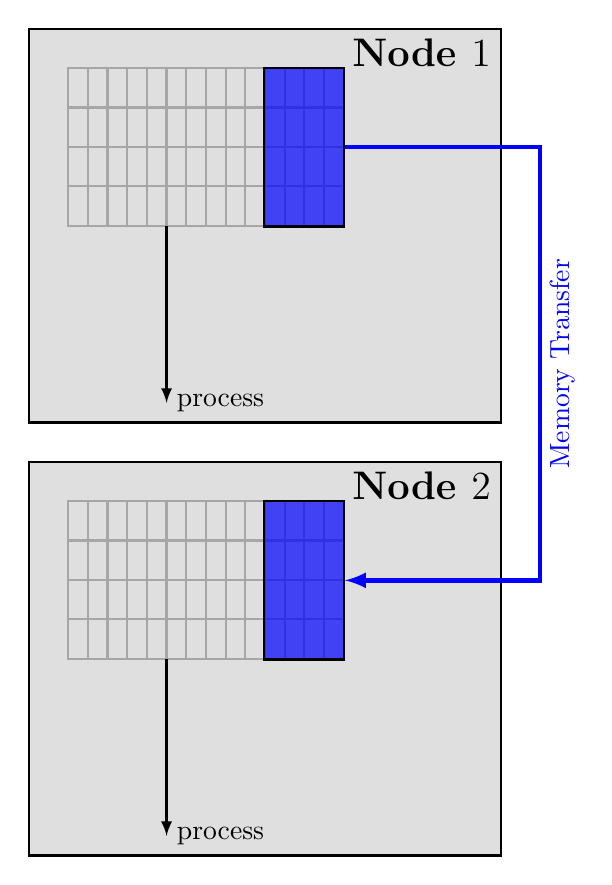
\begin{tikzpicture}

\draw[thick,fill=gray!25] (0,5.5) rectangle (6,10.5) node[anchor=north east,font=\Large] {\bfseries{}Node $1$};
\draw[thick,draw=gray!70] (.49,7.99) grid[xstep=.25cm,ystep=.5cm] (4,10.);
\draw[thick,fill=blue,fill opacity=.7] (2.99,7.99) rectangle (4,10.) node[fitting node] (n1) {};
\draw[thick,-latex] (1.75,8) -- (1.75,5.75) node[anchor=west] {process};

\draw[thick,fill=gray!25] (0,0) rectangle (6,5) node[anchor=north east,font=\Large] {\bfseries{}Node $2$};
\draw[thick,draw=gray!70] (.49,2.49) grid[xstep=.25cm,ystep=.5cm] (4,4.5);
\draw[thick,fill=blue,fill opacity=.7] (2.99,2.49) rectangle (4,4.5) node[fitting node] (n2) {};
\draw[thick,-latex] (1.75,2.5) -- (1.75,.25) node[anchor=west] {process};

\draw[ultra thick,blue,-latex] (n1.east) -- ($(n1) + (3cm,0)$) -- ($(n2) + (3cm,0)$) -- (n2.east);
\node (label) [text=blue,rotate=90,anchor=north] at($(n1)!.5!(n2) + (3cm,0)$) {Memory Transfer};
  \end{tikzpicture}
\end{document}
